\chapter{\uppercase{Experimental Setup}}

\begin{figure}[h!]
    \centering
    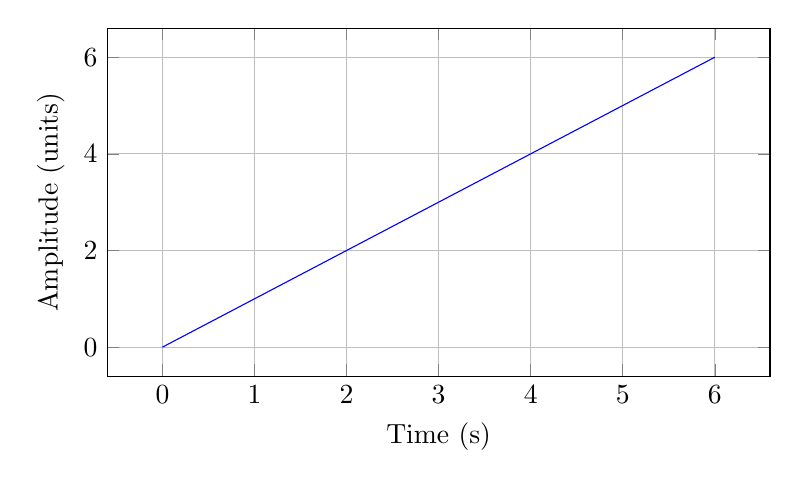
\begin{tikzpicture}
        \begin{axis}[
            xlabel={Time (s)},
            ylabel={Amplitude (units)},
            grid=major,
            width=10cm,
            height=6cm
        ]
        \addplot[
            domain=0:6,
            samples=100,
            color=blue
        ]{x};
        \end{axis}
    \end{tikzpicture}
    \caption{Amplitude as a function of time, demonstrating a linear increase.}
    \label{fig:time_vs_amplitude}
\end{figure}
Figure~\ref{fig:time_vs_amplitude} shows a simple example of amplitude varying linearly with time. This kind of plot is useful for illustrating the basic relationship between time and a measured quantity in controlled experiments \cite{kothari2004research}, \cite{weste2016cmosvlsi}, \cite{ozcan2016cognitive}, \cite{waldron2003generalized}, \cite{maedche2005ontology}. 
